\section{Analysis of the First Science Run}
\label{secRun08}

The data of the first science run has been acquired in 2010, between January 13 and June 8. About 2\% of the exposure has been rejected due to fluctuations in some detector operation parameters, such as pressure, temperature and liquid level, and 18 live days of data from April have been rejected due to an increased level of electronic noise. The total live time of the dataset used for dark matter search analysis is 100.9~days. In order to prevent any human bias in the analysis, this data has been blinded below S1~=~160~PE and the 90\% ER quantile in log$_{10}$(S2/S1) space. 

The analysis cuts (see Section~\ref{secDataQualityCuts}) have been designed based on $^{60}$Co, $^{137}$Cs and $^{241}$Am-Be calibration data, and the event vertex reconstruction algorithm based on NN has been used (see Chapter~\ref{chPositionReconstruction}). 
The energy region for the analysis has been defined from 4 to 30 PE. The lower bound is assumed to give a sufficient discrimination between S1 signals from particle interactions and electronic noise, and the upper bound includes most of the expected WIMP signal. 
Based on the parametrization of the relative scintillation efficiency described in Section~\ref{secLeff}, this region corresponds to nuclear recoil equivalent energy of 8.4$-$44.6~keV$_{\mathrm{nr}}$. The lower threshold decreased to slightly different $L_{eff}$ parametrization used in this analysis (see Section~\ref{secLeff}).

The total background expectation for the first science run is (1.8$\pm$0.6)~events, and is dominated by the $\beta$-decay of $^{85}$Kr (see Chapter~\ref{chERbackground}). The Gaussian leakage is predicted from the number of events in the `side band' (outside of the blinded dark matter search region), taking into account the blinding cut efficiency and the level of electronic recoil rejection. It is (1.14$\pm$0.48)~events in the WIMP search region, with error dominated by the statistical uncertainty in the definition of the discrimination line. 
The non-Gaussian (anomalous, `gamma-X') leakage (see Section~\ref{secConsistencyCuts}) is estimated using $^{60}$Co calibration data, taking into account the different exposure compared to background data. 
The expected anomalous leakage is (0.56$^{+0.21}_{-0.27}$)~events, with the uncertainty due to the difference in the background and calibration distributions, and due to uncertainty in the measurement of the krypton concentration. Since electrons have very short mean free path in liquid xenon, the $\beta$-decay of $^{85}$Kr does not contribute to this background source. 
The predicted nuclear recoil background from radiogenic and cosmogenic neutrons, taking into account the measured trigger efficiency and the energy threshold in the active veto, is (0.31$^{+0.22}_{-0.11}$)~events (see Section~\ref{secS2threshold}). With a correction for nuclear recoil acceptance due to S2/S1 electronic recoil discrimination cut, this results in (0.11$^{+0.08}_{-0.04}$)~events in the benchmark WIMP search region.
 
After unblinding the pre-defined signal region (Fig.~\ref{figRun08log10noise_1}), a population of events with low S2/S1 ratio has been observed below the 4~PE threshold, with 3 events leaking into the signal region, which is due to electronic pick-up noise. An example for one of these events is presented in Fig.~\ref{figRun08log10noise_2}, showing that a noise pulse has been misidentified as an S1 peak. Two cuts have been developed using calibration data, in order to reject events where the S1 peak is due to this electronic noise. One of them is a modified version of the 2-fold coincidence requirement for a valid S1 peak. If there is a contribution to S1 from two or more of the most noisy PMTs, the coincidence requirement is increased by the number of these PMTs. Additionally, not functioning PMT channels (Fig.~\ref{figPMTarrangement}) have also been used to reject this noise, since they do not detect any particle interaction but still pick up electronic noise. The second cut has been defined after unblinding, and is based on the width of the S1. The noise pulses are very narrow and can be efficiently rejected. 

\begin{figure}[!t]
\centering
\subfigure[]{
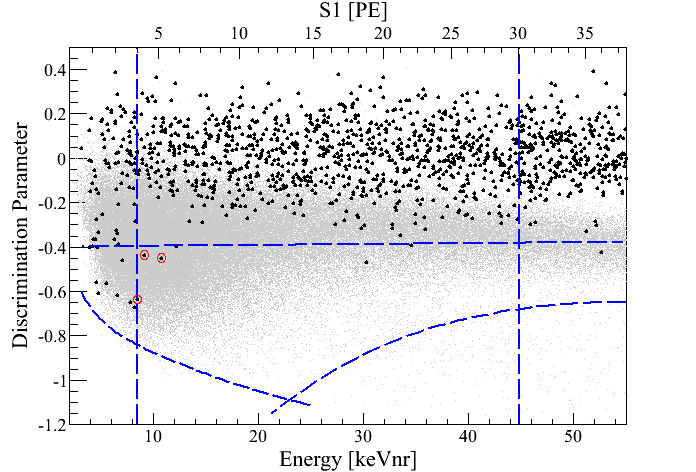
\includegraphics[width=0.475\linewidth]{plots/run08/run08_log10noise_withLabels1.png}
\label{figRun08log10noise_1}}
\subfigure[]{
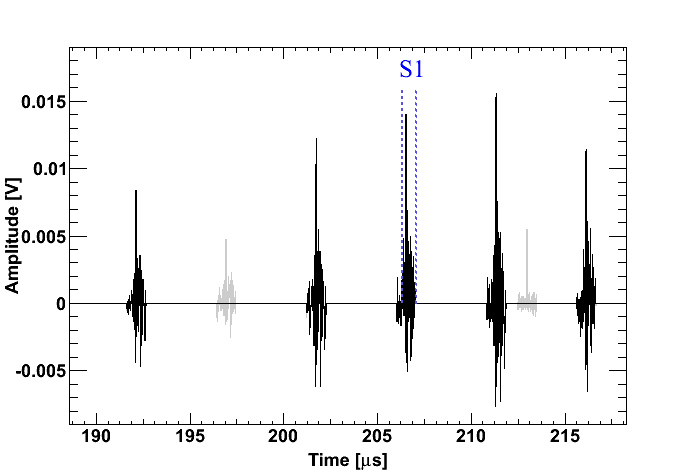
\includegraphics[width=0.475\linewidth]{plots/run08/run08_NoiseWaveform_mod1.png}
\label{figRun08log10noise_2}}
\caption[Distribution of events in the first science run using all cuts defined before unblinding the data]{(a) - distribution of events in the first science run using all cuts defined before unblinding the data. The population of events below 4~PE with 3 events leaking into the signal region (red circles) is due to electronic pick-up noise. 
(b) - an example waveform of a noise event remained in the signal region after the pre-defined cuts have been applied. The S1 identified by the peak finder algorithm is clearly due periodic electronic noise. The noise population is efficiently removed by the two new cuts defined post-unblinding.}
\label{figRun08log10noise}
\end{figure}

\begin{figure}[!b]
\centering
\subfigure[]{
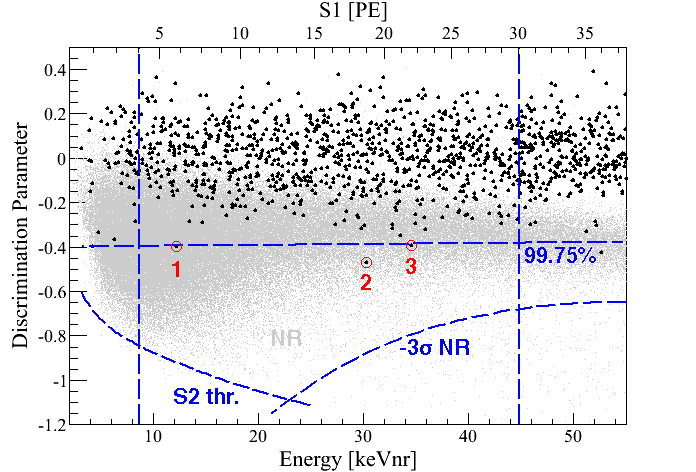
\includegraphics[width=0.475\linewidth]{plots/run08/run08_log10signal_withLabels1.png}
\label{figRun08log10signal_1}}
\subfigure[]{
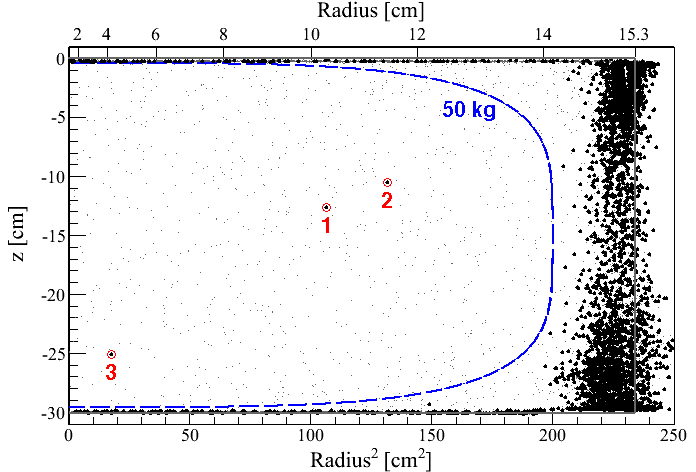
\includegraphics[width=0.475\linewidth]{plots/run08/run08_RZ_withLabels1.png}
\label{figRun08log10signal_2}}
\caption[Distribution of events in the first science run using all pre- and post-unblinding cuts]{(a) - distribution of events in log$_{10}$(S2/S1) space after applying all pre- and post-unblinding cuts. The noise population is rejected completely, and only three valid events are left in the signal region (marked with red circles). (b) - spatial distribution of all events (grey) and events in the signal region, below the 99.75\% ER rejection line (black) in the 8.4$-$44.6~keV$_{\mathrm{nr}}$ energy range. All pre- and post-unblinding cuts have been applied. The 48~kg fiducial volume is shown by the blue contour, and the dimensions of the target volume are indicated by the red lines.  Figures published in Ref.~\cite{xe100-run08}.}
\label{figRun08log10signal}
\end{figure}

\begin{figure}[!t]
\centering
\subfigure[Event 1: a clear and noise-free S1 signal is detected by PMTs 152 and 172. Electronic noise is present in waveform, but without any impact on the identified S1 signal, since the positions of the peaks are off from the noise frequency.]{
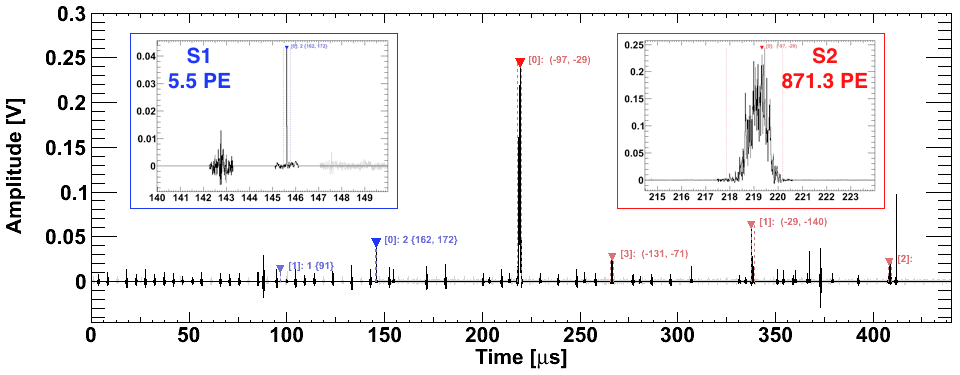
\includegraphics[width=0.92\linewidth]{plots/run08/event3.png}
\label{figRun08waveform_1}}
\subfigure[Event 2: a clear S1 peak is detected simultaneously by 6 PMTs. Electronic noise is not present in the waveform.]{
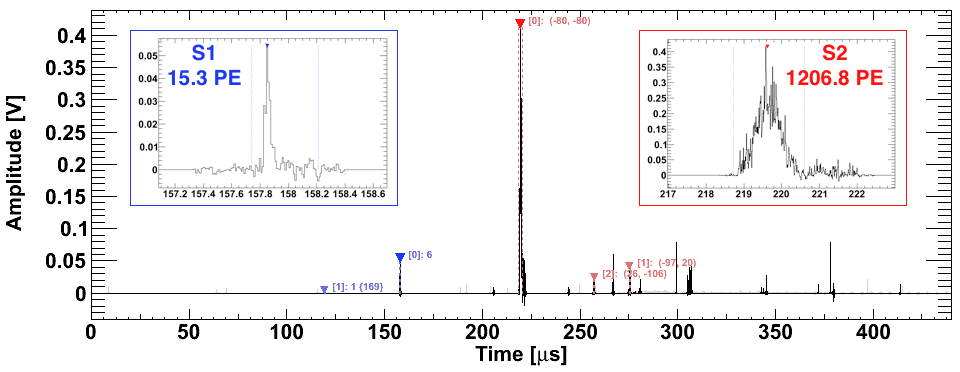
\includegraphics[width=0.92\linewidth]{plots/run08/event2.png}
\label{figRun08waveform_2}}
\subfigure[Event 3: a clear S1 signal with 16-fold coincidence. Periodic electronic noise is not present in waveform.]{
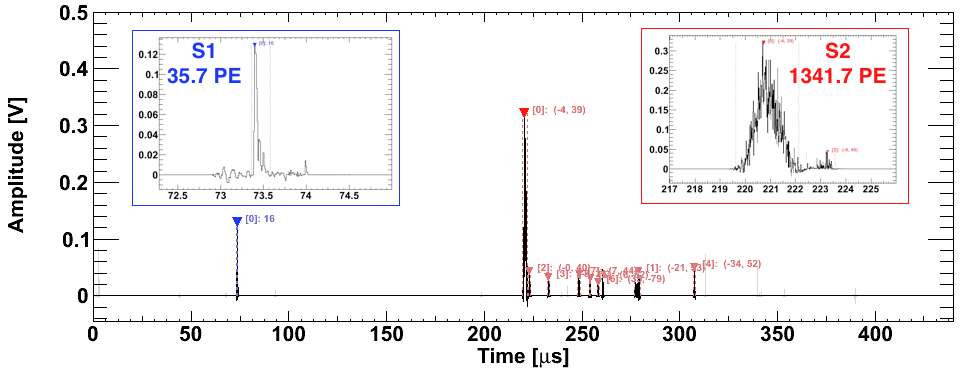
\includegraphics[width=0.92\linewidth]{plots/run08/event1.png}
\label{figRun08waveform_3}}
\caption[Waveforms of the signal candidate events of the first science run data]{Waveforms of the signal candidate events of the first science run data~\cite{xe100-run08}. The S1 peaks are labeled in blue, S2 peaks in red. The smaller peaks after the main S2 are from single ionization electrons extracted into the gas phase. The size of the S1 and S2 peaks refers to the values before the spatial corrections have been applied.}
\label{figRun08waveform}
\end{figure}

The distribution of events remaining after applying all pre- and post-unblinding data quality cuts is shown in Fig.~\ref{figRun08log10signal_1}. There are 3 events in the signal region (marked in red). The signal candidate events have been observed on January 23, February 12, and June 3, at 30.2~keV$_{\mathrm{nr}}$, 34.6~keV$_{\mathrm{nr}}$, and 12.1~keV$_{\mathrm{nr}}$, respectively. The spatial distribution in the target volume is shown in Fig.~\ref{figRun08log10signal_2}. 
Following the Poisson process, the probability  of the predicted (1.8$\pm$0.6)~background events to result in 3 or more events is 28\%. Hence, the observation of 3~events in the signal region does not constitute evidence for dark matter, and the result of this run is presented as a limit.

The waveforms of the signal candidate events are shown in Fig.~\ref{figRun08waveform}. The periodic electronic noise can be seen in the waveform of the lowest energy signal candidate event (event 1 in Fig.~\ref{figRun08log10signal}), as shown in in Fig.~\ref{figRun08waveform_1}, however, it does not affect a clear and unambiguous identification of the S1 peak. 

\begin{figure}[!b]
\centering
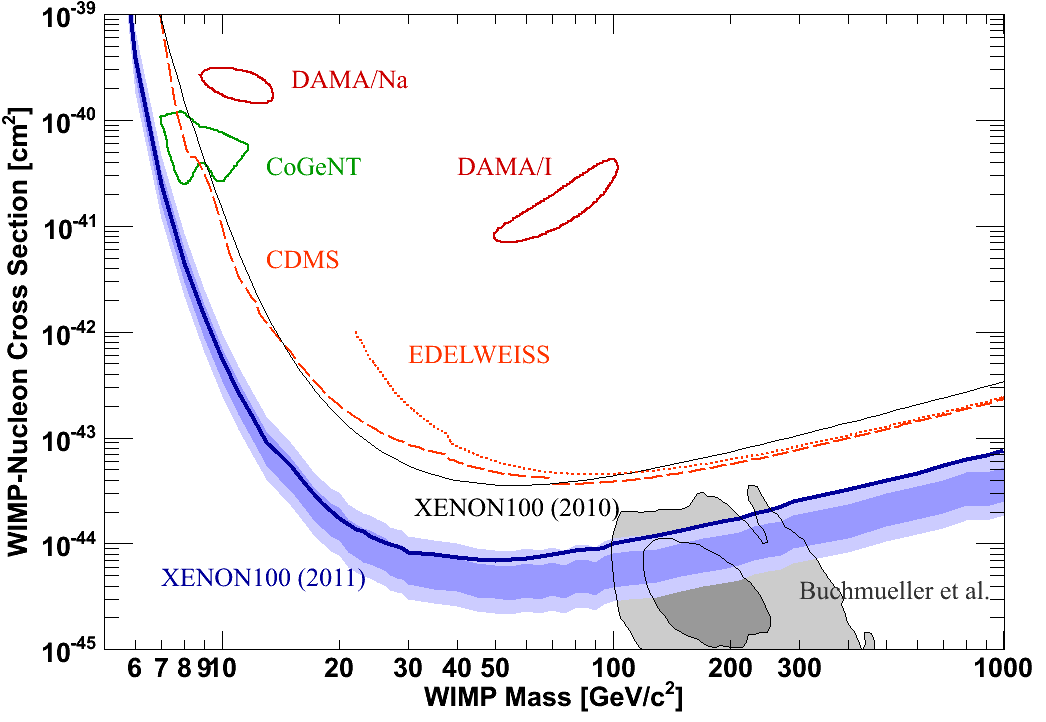
\includegraphics[width=0.6\linewidth]{plots/run08/run08_limit_mod.png}
\caption[Exclusion limit on spin-independent WIMP-nucleon scattering cross-section from the first science run]{Spin-independent elastic WIMP-nucleon scattering cross-section as a function of WIMP mass. The 90\% confidence limit (thick solid line) has been derived with the profile likelihood method~\cite{ProfileLikelihood}, taking into account all relevant systematic uncertainties. The 1$\sigma$ and 2$\sigma$ sensitivity of this run, calculated as the expected limit in absence of signal above background, is shown with the shaded bands. Also shown are the limits from the 11.17~live days of XENON100 data~(Section~\ref{secRun07}, lower 90\% C.L. $L_{eff}$), from CDMS~\cite{CDMS_limit}, and from EDELWEISS~\cite{EDELWEISS_limit} experiments. The expected parameter space from CMSSM~\cite{LHC} at 68\% and 95\% confidence level is indicated by the shaded gray regions. Figure published in Ref.~\cite{xe100-run08}.}
\label{figRun08limit}
\end{figure}

The calculation of the limit on the spin-independent WIMP-nucleon elastic scattering cross-section has been performed using the profile likelihood method~\cite{ProfileLikelihood}, which does not rely on s strict S2/S1 cut and provides higher acceptance to potential signal events. WIMPs are assumed to be distributed in an isothermal halo with a galactic rotation velocity of 220~km/s, a galactic escape velocity of 544$^{+64}_{-46}$~km/s, and a local density of 0.3~GeV/cm$^{3}$~\cite{LewinSmith, Smith}. The S1 resolution due to Poisson fluctuations has been taken into account. Uncertainties in the nuclear recoil energy scale (see Section~\ref{secLeff}), and the uncertainties in the galactic escape velocity have been profiled out and incorporated into the limit. 
The resulting limit at 90\% confidence level is shown in Fig.~\ref{figRun08limit}. The minimum cross-section is at 7.0$\times$10$^{-45}$~cm$^{2}$ at a WIMP mass of 50~GeV/c$^{2}$. The impact of $L_{eff}$ extrapolation below 3~keV$_{\mathrm{nr}}$ has been tested and is negligible at 10~GeV/c$^{2}$. The sensitivity of the XENON100 detector has been calculated as the expected limit in absence of signal above background and is also shown as 1$\sigma$ and 2$\sigma$ regions in Fig.~\ref{figRun08limit}. Due to the presence of two events around 30~keV$_{\mathrm{nr}}$, the limit at higher WIMP masses is slightly weaker than expected. This limit is consistent with the one from the standard (optimum interval) analysis~\cite{Yellin}, where the calculation is performed only on events in the WIMP search region. It has an acceptance-corrected exposure of 1471~kg$\cdot$days, when weighted with the spectrum of a 100~GeV/c$^{2}$ WIMP. This result excludes a large fraction of previously unexplored WIMP parameter space, being below all previous results, and cuts into the region where supersymmetric WIMP dark matter is accessible by the LHC~\cite{LHC}. It  severely constraints the interpretation of the DAMA~\cite{DAMA_LightWIMP} and CoGeNT~\cite{CoGeNT_LightWIMP, CoGeNT_modulation} signals as due to light mass ($<$20~GeV/c$^{2}$) WIMPs.

%The analysis has been performed with both optimum interval method~\cite{Yellin}, and with the profile likelihood analysis introduced in Ref.~\cite{ProfileLikelihood}.


%\begin{floatingfigure}[r]{0.475\textwidth}
%\begin{figure}[!h]
%\centering
%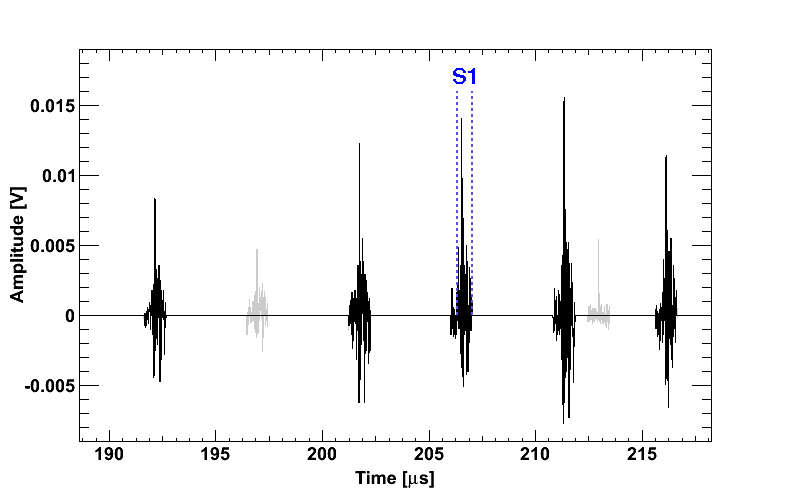
\includegraphics[width=0.475\linewidth]{plots/run08/run08_NoiseWaveform_mod_withLabels.png}
%\caption[An example waveform of a noise event remained in the signal region after the pre-defined cuts have been applied]{An example waveform of a noise event remained in the signal region after the pre-defined cuts have been applied. The S1 identified by the peak finder algorithm is clearly periodic electronic noise.}
%\label{figNoiseEvent}
%\end{figure}
%\end{floatingfigure}

%\begin{figure}[!h]
%\centering
%\subfigure[]{
%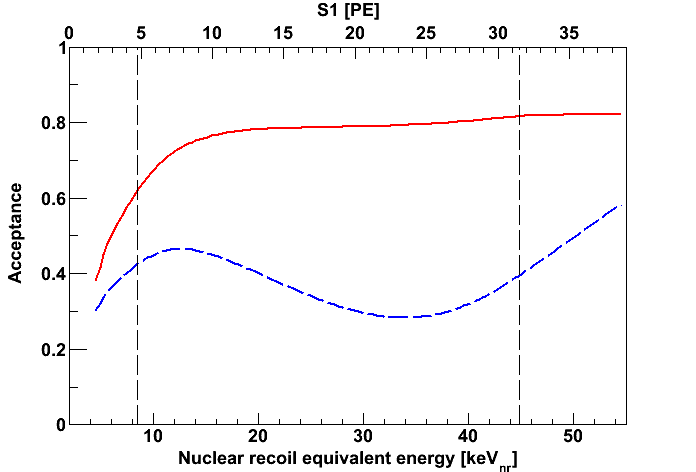
\includegraphics[width=0.475\linewidth]{plots/run08/run08_acceptance_mod.png}
%\label{figRun08rz_1}}
%\subfigure[]{
%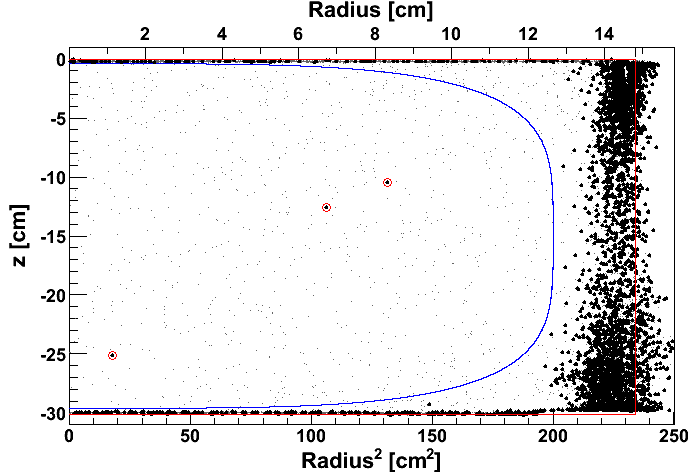
\includegraphics[width=0.475\linewidth]{plots/run08/run08_RZ_mod.png}
%\label{figRun08rz_2}}
%\caption[Acceptance ]{(a) - acceptance of all data quality cuts used for the analysis of the first science run (red), excluding the S2/S1 discrimination cut, and nuclear recoil acceptance for 99.75\% electronic recoil rejection cut (blue). (b) - spatial distribution of all events (grey) and events in the signal region, below 99.75\% ER rejection line (black) in the TPC observed in the 8.4$-$44.6~keV$_{nr}$ energy range. All pre- and post-unblinding cuts have been applied. The 48~kg fiducial volume is shown with the blue line, and the dimensions of the target volume are indicated with the red lines.}
%\label{figRun08rz}
%\end{figure}


%\begin{figure}[!h]
%\centering
%\subfigure[S1 light pattern]{
%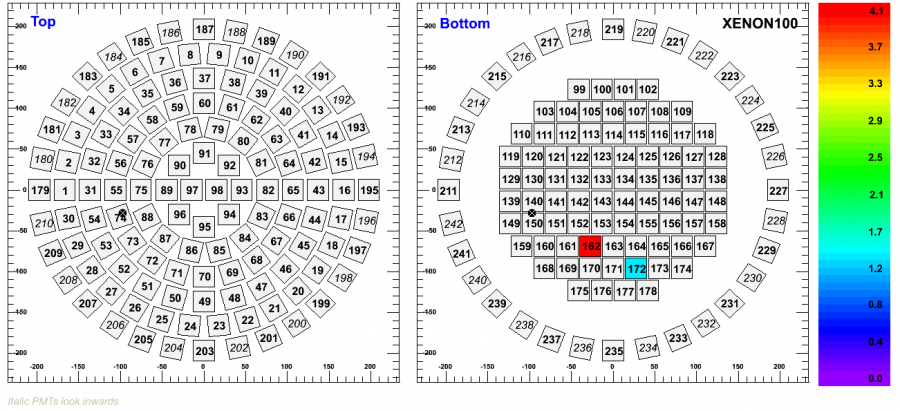
\includegraphics[width=0.8\linewidth]{plots/run08/run08_1event_patternS1.png}
%\label{figRun08pattern_1}}
%\subfigure[S2 light pattern]{
%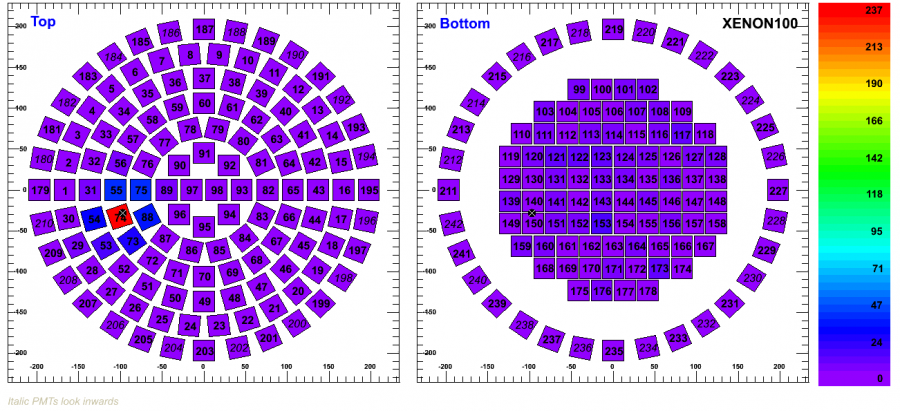
\includegraphics[width=0.8\linewidth]{plots/run08/run08_1event_patternS2.png}
%\label{figRun08pattern_2}}
%\caption[Light patterns of the S1 and S2 signals for the lowest energy signal candidate event]{Light patterns of the S1 and S2 signals for the lowest energy signal candidate event. The position of the interaction, reconstructed with the algorithm based on neural network, is shown with a black circle. }
%\label{figRun08pattern}
%\end{figure}

